% !TeX root = ../tfg.tex
% !TeX encoding = utf8

\chapter{Irregularidades en la Dinámica del Error}\label{ap:apendiceD}

En este apéndice analizamos en detalle los saltos bruscos que se producen tanto en el error de entrenamiento como en el de test al aumentar el número de épocas de un determinado modelo, intentando proporcionar una explicación para los mismos.\newline

Nos centramos en la gráfica de la Figura~\ref{fig:model-epoch3CNNCIFAR10}, donde estos picos en el error son más sobresalientes. A partir de esta representación, se analiza el \textit{epoch-wise double descent} en dos modelos que la conforman: uno infraparametrizado, ubicado antes del umbral de interpolación, y otro sobreparametrizado, situado después de dicho umbral.\newline

\begin{figure}[h]
    \centering
    \begin{subfigure}[b]{\textwidth}
        \centering
        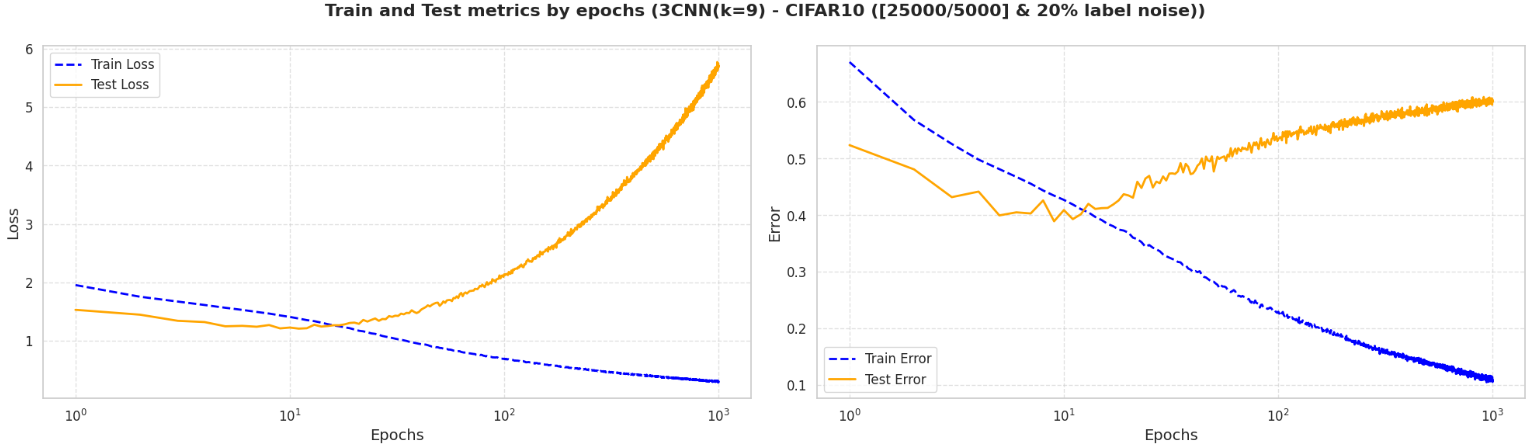
\includegraphics[width=0.9\textwidth]{img/experiments/epoch-wise3CNNunderparameterized.png}
        \caption{A la izquierda, se muestra la pérdida en entrenamiento y test, y a la derecha, el error en entrenamiento y test para un modelo $3$CNN infraparametrizado ($k=9$) sobre el subconjunto CIFAR$10$[$25000/5000$], con $20\%$ de ruido añadido y un \text{batch size} de $128$.}\label{fig:epoch-wise3CNNunderparameterized}
    \end{subfigure}
    
    \vspace{1em} 

    \begin{subfigure}[b]{\textwidth}
        \centering
        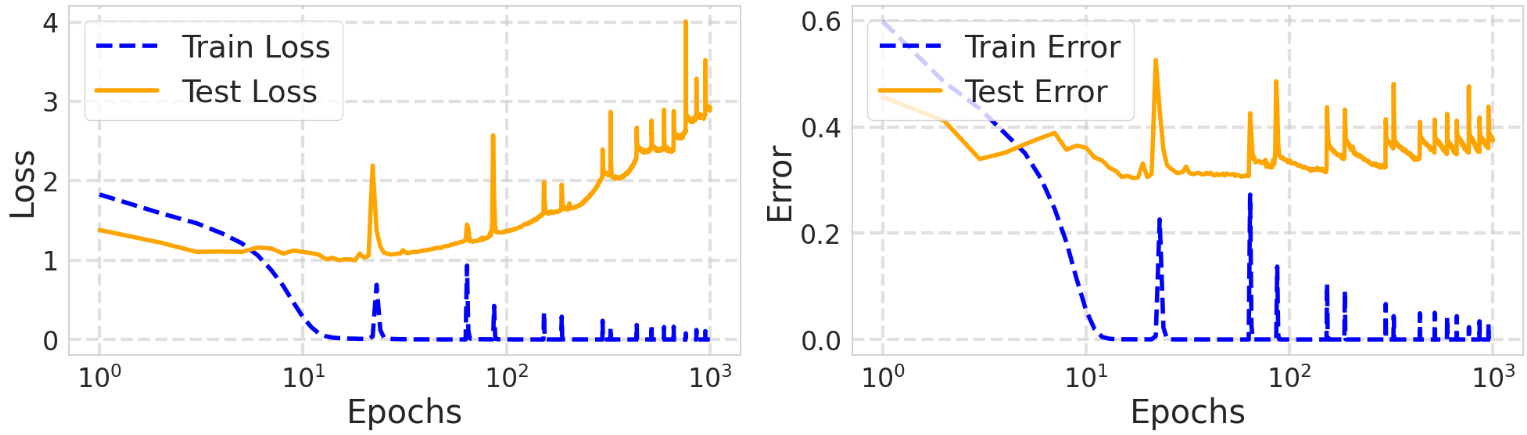
\includegraphics[width=0.9\textwidth]{img/experiments/epoch-wise3CNNoverparameterized.png}
        \caption{A la izquierda, se muestra la pérdida en entrenamiento y test, y a la derecha, el error en entrenamiento y test para un modelo $3$CNN sobreparametrizado ($k=60$) sobre el subconjunto CIFAR$10$[$25000/5000$], con $20\%$ de ruido añadido y un \text{batch size} de $128$. Se aprecian variaciones abruptas tanto en la gráfica de la pérdida como en la del error.}\label{fig:epoch-wise3CNNoverparameterized}
    \end{subfigure}
    
    \caption[Comparativa \textit{epoch-wise double descent} entre un modelo infraparametrizado y uno sobreparametrizado en el que aparecen picos significativos en el error.]{Comparativa \textit{epoch-wise double descent} entre un modelo infraparametrizado, donde no se observa el doble descenso, y un modelo sobreparametrizado, en el que este efecto sí se manifiesta y aparecen picos significativos en el error.}\label{fig:epoch-wise-bruscos1}
\end{figure}

Para intentar dar una explicación coherente a la conducta, ciertamente peculiar, que se observa en estas gráficas, recordemos algunos de los resultados presentados en la Sección~\ref{sec:optimizacion-zona-sobreparametrizada}. En la zona infraparametrizada, sabemos que los mínimos locales suelen estar aislados, lo que provoca que el paisaje de la función de pérdida en sus alrededores sea localmente convexo (véase imagen izquierda de la Figura~\ref{fig:localglobalminima}).\newline

Debido a esto, la inicialización del optimizador juega un papel crucial, ya que determinará hacia qué mínimo local convergerá. En particular, el optimizador tiende a dirigirse hacia el mínimo local más cercano a su punto de inicio. Dado que la región circundante es localmente convexa, el optimizador avanzará progresivamente hacia dicho mínimo sin posibilidad de escapar de él, siempre que la tasa de aprendizaje sea adecuada. Este comportamiento explica por qué, en la zona infraparametrizada, la pérdida en entrenamiento sigue una tendencia descendente y converge de manera estable. Al no haber direcciones de escape significativas, el optimizador se mantiene atrapado en el mínimo local alcanzado, lo que se traduce en una reducción progresiva y sostenida de la pérdida a lo largo del proceso de optimización. Sin embargo, debido a la limitada capacidad del modelo en esta región, el error en el conjunto de test permanece elevado, reflejando una falta de flexibilidad para ajustarse adecuadamente a los datos (véase Figura~\ref{fig:epoch-wise3CNNunderparameterized}).\newline

En cambio, en la zona sobreparametrizada, los mínimos globales no están aislados, sino que en cualquier pequeña vecindad de ellos siempre es posible encontrar otro minimizador global (véase Sección~\ref{sec:optimizacion-zona-sobreparametrizada}). Esto implica que la función de pérdida presenta una alta no convexidad, incluso a nivel local. Como resultado, el paisaje de la función de pérdida en estos modelos es multimodal, como se ilustra en la imagen izquierda de la Figura~\ref{fig:landscapes}. Aunque dicha imagen muestre únicamente un mínimo global en un espacio tridimensional, es importante recordar que existen múltiples de ellos en las dimensiones definidas por el espacio de parámetros. En otras palabras, paisajes similares a este (aunque más complejos debido a su alta dimensionalidad) se replicarían en distintas regiones del espacio de parámetros, dando lugar a un paisaje altamente multimodal con una multitud de mínimos globales.\newline 

\begin{figure}[h!]
    \centering
    \begin{minipage}{0.49\textwidth}
        \centering
        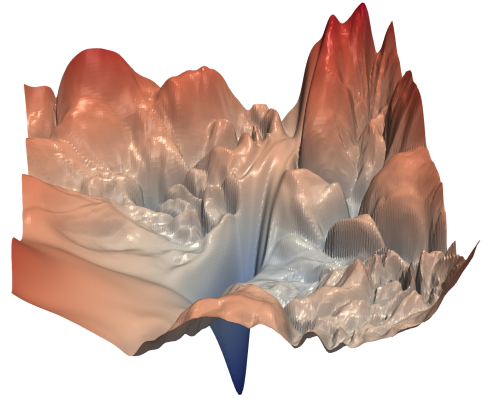
\includegraphics[width=\linewidth]{img/experiments/landscapemultimodal.png}
    \end{minipage}
    \hfill
    \begin{minipage}{0.49\textwidth}
        \centering
        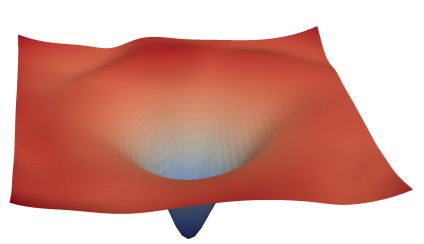
\includegraphics[width=\linewidth]{img/experiments/landscapeunimodal.png}
    \end{minipage}
    \caption[Paisajes de la función de pérdida para distintos modelos sobreparametrizados~\cite{Li2018}.]{Paisajes de la función de pérdida para un modelo sobreparametrizado sin conexiones residuales (izquierda) y con conexiones residuales (derecha)~\cite{Li2018}. A la izquierda, se observa un único mínimo global en un entorno altamente multimodal. A la derecha, se observa un único mínimo global en un entorno unimodal, fruto de las conexiones residuales.}\label{fig:landscapes}
\end{figure} 

A partir de estos resultados, podemos inferir que el algoritmo de optimización, una vez ha alcanzado una solución prácticamente perfecta (es decir, al encontrar un mínimo, potencialmente global, de la función de pérdida), continúa explorando en busca de soluciones aún mejores (en términos de generalización). Este proceso, debido a la naturaleza del paisaje multimodal en el que opera, provoca que el modelo pueda salir de dicho mínimo, lo que da lugar a los picos observados, para luego converger hacia otro mínimo potencialmente global.\newline

Además, otro hecho relevante es que la magnitud de estos saltos disminuye progresivamente, lo que sugiere que el modelo, al buscar nuevos mínimos globales, tiende a seleccionar un tipo de soluciones frente a otras. Esta respuesta del modelo puede asociarse al hecho de que, entre todas las soluciones posibles, busca aquella que sea más simple, lo cual, como se ha observado en experimentos previos, suele ser una solución que generaliza bien.\newline

La pregunta ahora sería por qué hemos observado estos resultados, cuando no se muestran de manera prominente en la literatura científica. En primer lugar, en los estudios que presentan gráficas de error con el fenómeno del doble descenso, generalmente se utilizan arquitecturas que incluyen conexiones residuales. Este tipo de arquitecturas, según lo demuestran Li et al.~\cite{Li2018}, no presentan paisajes de la función de pérdida multimodales. En cambio, exhiben zonas planas alrededor de los mínimos, impidiendo los saltos bruscos observados en nuestro caso (véase imagen derecha de la Figura~\ref{fig:landscapes}). Así, los mínimos globales se asemejan a los mínimos locales de las zonas infraparametrizadas, lo que impide que el algoritmo de optimización escape de ellos.\newline

Por otra parte, siguiendo los distintos resultados presentados en la Sección~\ref{subsec:model-epoch-wise}, podemos observar que el aumento en el número de parámetros en comparación con el número de ejemplos de entrenamiento, junto con el uso de un conjunto de entrenamiento más difícil (en nuestro caso, conjuntos con imágenes en formato RGB), favorecen la aparición de estas colinas en las gráficas de error.\newline

Finalmente, podemos concluir que, a medida que avanzan las épocas de entrenamiento, estos picos se vuelven cada vez menos notables, posiblemente porque el modelo encuentra cada vez soluciones más simples. Esto sugiere que, si se entrenara durante un mayor número de épocas de entrenamiento, estos picos podrían llegar a ser prácticamente imperceptibles o incluso desaparecer por completo.\newline

\endinput
%------------------------------------------------------------------------------------
% FIN DEL APÉNDICE. 
%------------------------------------------------------------------------------------
